% Options for packages loaded elsewhere
\PassOptionsToPackage{unicode}{hyperref}
\PassOptionsToPackage{hyphens}{url}
\PassOptionsToPackage{dvipsnames,svgnames,x11names}{xcolor}
%
\documentclass[
  10pt,
  ignorenonframetext,
]{beamer}
\usepackage{pgfpages}
\setbeamertemplate{caption}[numbered]
\setbeamertemplate{caption label separator}{: }
\setbeamercolor{caption name}{fg=normal text.fg}
\beamertemplatenavigationsymbolsempty
% Prevent slide breaks in the middle of a paragraph
\widowpenalties 1 10000
\raggedbottom
\setbeamertemplate{part page}{
  \centering
  \begin{beamercolorbox}[sep=16pt,center]{part title}
    \usebeamerfont{part title}\insertpart\par
  \end{beamercolorbox}
}
\setbeamertemplate{section page}{
  \centering
  \begin{beamercolorbox}[sep=12pt,center]{part title}
    \usebeamerfont{section title}\insertsection\par
  \end{beamercolorbox}
}
\setbeamertemplate{subsection page}{
  \centering
  \begin{beamercolorbox}[sep=8pt,center]{part title}
    \usebeamerfont{subsection title}\insertsubsection\par
  \end{beamercolorbox}
}
\AtBeginPart{
  \frame{\partpage}
}
\AtBeginSection{
  \ifbibliography
  \else
    \frame{\sectionpage}
  \fi
}
\AtBeginSubsection{
  \frame{\subsectionpage}
}
\usepackage{amsmath,amssymb}
\usepackage{iftex}
\ifPDFTeX
  \usepackage[T1]{fontenc}
  \usepackage[utf8]{inputenc}
  \usepackage{textcomp} % provide euro and other symbols
\else % if luatex or xetex
  \usepackage{unicode-math} % this also loads fontspec
  \defaultfontfeatures{Scale=MatchLowercase}
  \defaultfontfeatures[\rmfamily]{Ligatures=TeX,Scale=1}
\fi
\usepackage{lmodern}
\usetheme[]{metropolis}
\ifPDFTeX\else
  % xetex/luatex font selection
\fi
% Use upquote if available, for straight quotes in verbatim environments
\IfFileExists{upquote.sty}{\usepackage{upquote}}{}
\IfFileExists{microtype.sty}{% use microtype if available
  \usepackage[]{microtype}
  \UseMicrotypeSet[protrusion]{basicmath} % disable protrusion for tt fonts
}{}
\makeatletter
\@ifundefined{KOMAClassName}{% if non-KOMA class
  \IfFileExists{parskip.sty}{%
    \usepackage{parskip}
  }{% else
    \setlength{\parindent}{0pt}
    \setlength{\parskip}{6pt plus 2pt minus 1pt}}
}{% if KOMA class
  \KOMAoptions{parskip=half}}
\makeatother
\usepackage{xcolor}
\newif\ifbibliography
\usepackage{listings}
\newcommand{\passthrough}[1]{#1}
\lstset{defaultdialect=[5.3]Lua}
\lstset{defaultdialect=[x86masm]Assembler}
\usepackage{graphicx}
\makeatletter
\def\maxwidth{\ifdim\Gin@nat@width>\linewidth\linewidth\else\Gin@nat@width\fi}
\def\maxheight{\ifdim\Gin@nat@height>\textheight\textheight\else\Gin@nat@height\fi}
\makeatother
% Scale images if necessary, so that they will not overflow the page
% margins by default, and it is still possible to overwrite the defaults
% using explicit options in \includegraphics[width, height, ...]{}
\setkeys{Gin}{width=\maxwidth,height=\maxheight,keepaspectratio}
% Set default figure placement to htbp
\makeatletter
\def\fps@figure{htbp}
\makeatother
\setlength{\emergencystretch}{3em} % prevent overfull lines
\providecommand{\tightlist}{%
  \setlength{\itemsep}{0pt}\setlength{\parskip}{0pt}}
\setcounter{secnumdepth}{-\maxdimen} % remove section numbering
\ifLuaTeX
\usepackage[bidi=basic]{babel}
\else
\usepackage[bidi=default]{babel}
\fi
\babelprovide[main,import]{american}
% get rid of language-specific shorthands (see #6817):
\let\LanguageShortHands\languageshorthands
\def\languageshorthands#1{}
\usepackage{fancyhdr}
\pagestyle{fancy}
\usepackage{setspace}
\usepackage{graphicx}
\usepackage{amsfonts}
\usepackage{amssymb}
\usepackage{amsmath}
\usepackage{minted}
\ifLuaTeX
  \usepackage{selnolig}  % disable illegal ligatures
\fi
\IfFileExists{bookmark.sty}{\usepackage{bookmark}}{\usepackage{hyperref}}
\IfFileExists{xurl.sty}{\usepackage{xurl}}{} % add URL line breaks if available
\urlstyle{same}
\hypersetup{
  pdftitle={Understanding Memory Management},
  pdfauthor={Dipesh Kafle},
  pdflang={en-US},
  colorlinks=true,
  linkcolor={blue},
  filecolor={Maroon},
  citecolor={Blue},
  urlcolor={red},
  pdfcreator={LaTeX via pandoc}}

\title{Understanding Memory Management}
\author{Dipesh Kafle}
\date{}

\begin{document}
\frame{\titlepage}

\hypertarget{prerequisites}{%
\section{Prerequisites}\label{prerequisites}}

\begin{frame}{Memory Layout}
\protect\hypertarget{memory-layout}{}
\begin{figure}
\centering
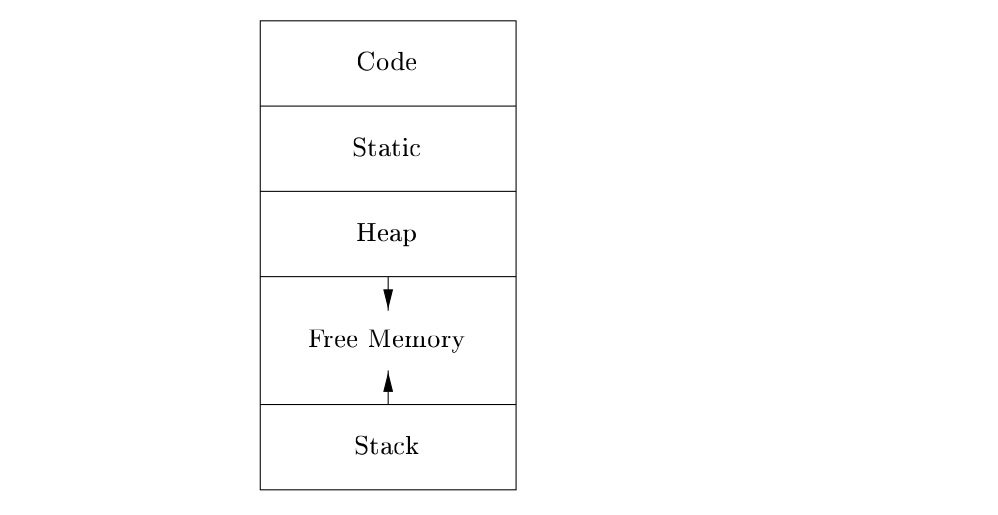
\includegraphics[width=0.5\textwidth,height=\textheight]{memory.png}
\caption{A program's memory segments roughly
classified}
\end{figure}

\begin{itemize}
\tightlist
\item
  In practice, the stack grows towards lower
  addresses, the heap towards higher(the diagram
  has it the other way around, but that doesn't
  matter).
\end{itemize}

\pause

\begin{itemize}
\tightlist
\item
  What are all these things ??
\end{itemize}

\pause

\begin{itemize}
\tightlist
\item
  We are mainly concerned withe the stack and the
  heap for the purpose of this talk, but we'll see
  what the other things are as well.
\end{itemize}
\end{frame}

\begin{frame}[fragile]{Code and Static segments}
\protect\hypertarget{code-and-static-segments}{}
\begin{itemize}
\tightlist
\item
  Code : The size of the generated target code is
  fixed at compile time, so the compiler can place
  the executable target code in a statically
  determined area Code, usually in the low end of
  memory.
\end{itemize}

\pause

\begin{itemize}
\tightlist
\item
  Static : The size of some program data objects,
  such as global constants, and data generated by
  the compiler that may be known at compile time,
  and these data objects can be placed in another
  statically determined area called Static.
\end{itemize}

\pause

\begin{minted}{cpp}
const char* s = "Lorem Ipsum something something";
int main(){
  const char* string_arr[] = {"Made", "with", "love", "by", "Delta", "Force"};
  return 0;
}
\end{minted}

All the strings used in the above code segment are
stored in static section, while the instructions
generated for the program will be in code section.
\end{frame}

\begin{frame}[fragile]{Stack and Stack Allocation}
\protect\hypertarget{stack-and-stack-allocation}{}
\begin{itemize}
\tightlist
\item
  The stack will store things such as local
  variables, return address from a function call,
  etc.
\end{itemize}

\begin{lstlisting}[language=C]
int main(){
  int a = 10; // This is doing stack allocation
  int b = 20;
  int arr[2] = {1,2};
  return 0;
}
\end{lstlisting}

\begin{figure}
\centering
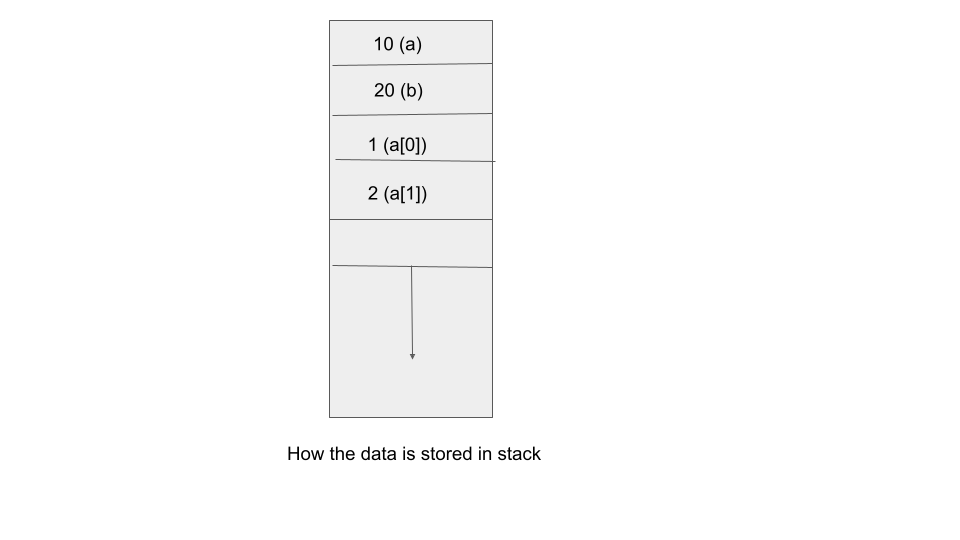
\includegraphics[width=0.5\textwidth,height=\textheight]{stack_layout.png}
\caption{Stack Layout for above code}
\end{figure}
\end{frame}

\begin{frame}[fragile]{Heap and Heap Allocation}
\protect\hypertarget{heap-and-heap-allocation}{}
\begin{itemize}
\tightlist
\item
  Many programming languages allow the programmer
  to allocate and deallocate data under program
  control.
\end{itemize}

\pause

\begin{itemize}
\tightlist
\item
  The heap is used to manage long-lived data.
\end{itemize}

\pause

\begin{itemize}
\tightlist
\item
  C/C++ has malloc/realloc/free functions for
  doing heap memory management.
\end{itemize}

\pause

\begin{itemize}
\tightlist
\item
  Unavoidable when we want to allocate memory
  whose size is known only when the program is
  running(dynamic allocation).
\end{itemize}

\pause

\begin{lstlisting}[language=C]
int* f(){
  return malloc(10*sizeof(int));
}
int main(){
   int n ;
   scanf("%d", &n);
   int *arr = f(); // arr is heap allocated,returned from call to f
   free(arr); //Since, we're good programmers, we'll free the memory as well.
}
\end{lstlisting}
\end{frame}

\begin{frame}[fragile]{What exactly are
malloc/realloc/free?}
\protect\hypertarget{what-exactly-are-mallocreallocfree}{}
\begin{itemize}
\tightlist
\item
  They're just functions that help us with heap
  allocation
\item
  We call \passthrough{\lstinline!malloc!} with
  argument \passthrough{\lstinline!x!} when we
  want to allocate \passthrough{\lstinline!x!}
  number of bytes we want to allocate in heap.
\item
  We call \passthrough{\lstinline!realloc!} when
  we want to increase the size of previously
  allocated heap memory. One possible reason for
  using this is for resizing an array.
\item
  We call \passthrough{\lstinline!free!} when we
  are done with the heap allocated memory and we
  want to return it back to the operating system.
\end{itemize}
\end{frame}

\hypertarget{introduction-to-memory-management}{%
\section{Introduction to Memory
Management}\label{introduction-to-memory-management}}

\begin{frame}{Introduction to Memory Management}
\begin{itemize}
\tightlist
\item
  Memory Management is mainly just the act of
  allocating heap memory and freeing them
  appropriately.
\end{itemize}

\pause

\begin{itemize}
\tightlist
\item
  Stack allocations need not be freed, it's
  managed automatically with \textbf{scopes}(we'll
  see what scope means in next slide).
\end{itemize}

\pause

\begin{block}{Important terminology}
\protect\hypertarget{important-terminology}{}
\begin{itemize}
\tightlist
\item
  Memory Leak: It happens when you ask the
  operating system for memory but don't return it
  back.
\end{itemize}
\end{block}
\end{frame}

\begin{frame}[fragile]{What is this scope thing??}
\protect\hypertarget{what-is-this-scope-thing}{}
\begin{lstlisting}[language=C]
// NOTE: This function won't compile
int f(){ // scope '1 starts
    int a = 10;
    { // scope '2 starts
       int b = 20;
    } // scope '2 ends
    if(a == 10){ scope '3 starts
      int c = 30;
    } // scope '3 ends
    return b; // This fails because it's not in scope
} // scope '1 ends
\end{lstlisting}
\end{frame}

\begin{frame}{Why should I care about freeing
memory? Is it really a problem?}
\protect\hypertarget{why-should-i-care-about-freeing-memory-is-it-really-a-problem}{}
\begin{itemize}
\tightlist
\item
  You don't need to care if you have infinite
  memory in your system. But sadly, there is only
  finite memory.
\end{itemize}

\pause

\begin{itemize}
\tightlist
\item
  If one program takes up all the memory, other
  programs(that may require memory) won't be able
  to progress normally.
\end{itemize}

\pause

\begin{itemize}
\tightlist
\item
  Your program may crash if it asks for more
  memory that the operating system can provide.
\end{itemize}

\pause

\begin{itemize}
\tightlist
\item
  Memory leaks will especially affect long running
  programs such as web servers, editors, IDEs,
  etc.
\end{itemize}
\end{frame}

\hypertarget{ways-to-manage-memory}{%
\section{Ways to manage
memory}\label{ways-to-manage-memory}}

\begin{frame}{Ways to manage memory}
We have two ways to do memory management.

\pause

\begin{itemize}
\item
  \textbf{Manual Memory Management} : Languages
  such as C, C++, Rust, etc have this
\item
  \textbf{Automatic Memory Management}: Languages
  such as Python, Java, Go, JavaScript, Swift, etc
  have this.
\end{itemize}
\end{frame}

\hypertarget{manual-memory-management}{%
\section{Manual Memory
Management}\label{manual-memory-management}}

\hypertarget{introduction-to-automatic-memory-management}{%
\section{Introduction to Automatic Memory
Management}\label{introduction-to-automatic-memory-management}}

\hypertarget{reference-counting}{%
\section{Reference
Counting}\label{reference-counting}}

\hypertarget{trace-based-collection}{%
\section{Trace Based
Collection}\label{trace-based-collection}}

\hypertarget{which-is-betterautomatic-memory-management-or-manual-management}{%
\section{Which is better?(Automatic Memory
Management or Manual
Management}\label{which-is-betterautomatic-memory-management-or-manual-management}}

\hypertarget{advanced-topics-in-garbage-collection}{%
\section{Advanced Topics in Garbage
Collection}\label{advanced-topics-in-garbage-collection}}

\begin{frame}{Advanced Topics in Garbage
Collection}
\begin{itemize}
\item
  Incremental GC
\item
  Parallel and Concurrent GC
\item
  Precise and Conservative Garbage Collectors
\item
  Reducing GC pause*
\end{itemize}
\end{frame}

\hypertarget{references}{%
\section{References}\label{references}}

\begin{frame}{References}
\begin{itemize}
\tightlist
\item
  \href{https://rebelsky.cs.grinnell.edu/Courses/CS302/99S/Presentations/GC/}{Some
  presentation on GC, Grinnel college}
\end{itemize}
\end{frame}

\end{document}
